\subsection{Diagramme d'Activité et Objet de Flux}

Le diagramme d’activité est attaché à une catégorie de classe et décrit le déroulement des activités de cette catégorie. Il indique la part prise par chaque objet dans
l’exécution d’un travail.

Objet de flux est un connecteur avec une pointe de flèche dénotant la direction ou on passe l’objet. Il doit avoir un objet sur au moins une de ses fins. 
Ce diagramme d'activité sera lié au processus effectuer commende.



\begin{minipage}{1\textwidth}
	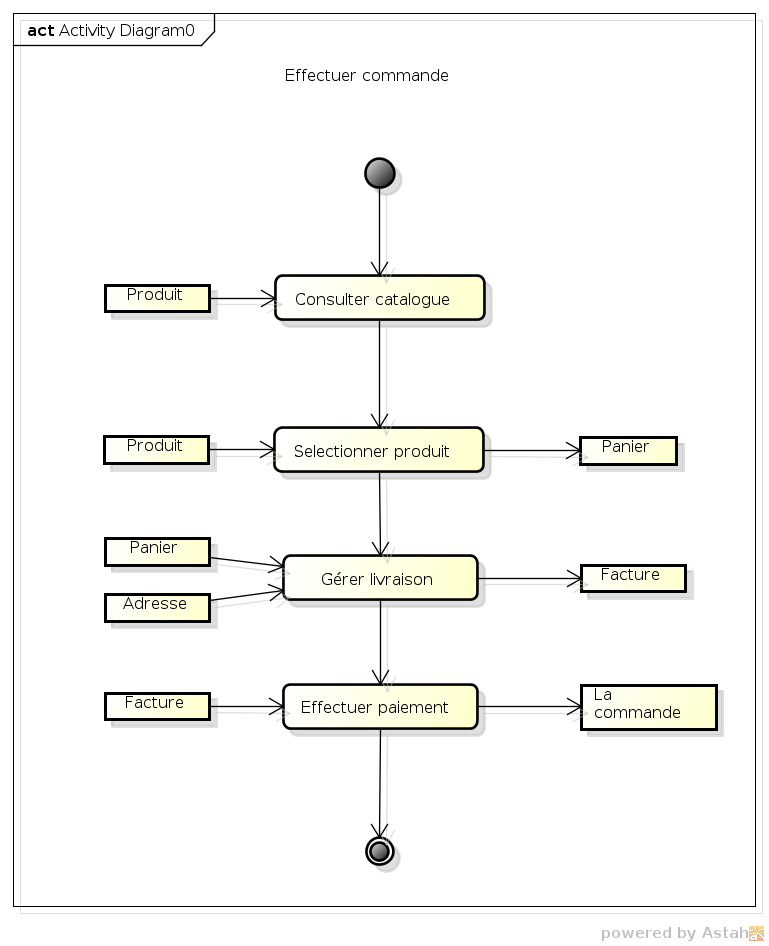
\includegraphics[width=0.7\linewidth]{mama/images/Effectuer}
	\label{fig:Effectuer}
\end{minipage}
\hspace*{\stretch{1}}

Le diagramme d’activité est un Diagramme associé à un objet particulier ou à un ensemble d’objets, qui illustre les flux entre les activités et les actions. Il permet de représenter graphiquement le déroulement d’un cas d’utilisation métier sur les commandes.



